\documentclass[11pt]{article}

\usepackage[pdftex]{graphicx} % OU
% \usepackage[dvips]{graphicx}

% \usepackage[round]{natbib}
\usepackage{adjustbox,array,url,hyperref,multirow,makecell,tabularx,caption,subcaption}
% \usepackage{url,hyperref,multirow,makecell}
\usepackage[table]{xcolor}
\usepackage{lipsum}
\usepackage{cite}
\usepackage{amsfonts}
%\usepackage[latin1]{inputenc}
\usepackage[utf8]{inputenc}
%\usepackage[brazilian,brazil]{babel}
%\usepackage{apacite}
%\usepackage{float}
\usepackage{booktabs}
\usepackage{multirow}

\usepackage{todonotes}
\newcommand{\pmendes}[1]{\color{blue}\textbf{paulo says: }#1\color{black}}

\usepackage{tikz}
\usetikzlibrary{
  angles,
  arrows,
  arrows.meta,
  calc,
  intersections,
  positioning,
  quotes,
  shapes.geometric,
  through,
}
\tikzset{
  x=0em,
  y=0em,
  node distance=1.2em,
  >=stealth',
}

\newcommand*\rot[1]{\rotatebox{90}{#1}}

\newtheorem{proposition}{Proposition}
\newtheorem{lemma}{Lemma}
\newtheorem{theorem}{Theorem}

\newcommand{\CQD}{\mbox{\rule[0pt]{1.5ex}{1.5ex}}\medskip}
\newcommand{\M}{\mathcal{M}}

\setlength{\oddsidemargin}{0.5cm} \setlength{\textwidth}{15cm}
\setlength{\topmargin}{-1.5cm} \setlength{\textheight}{22.3cm}%{24.7cm}

\usepackage{pdfpages}

\begin{document}

\LARGE

% \bigskip

%% TITLE
\begin{center}
{\bf Spatiotemporal Localization of Actors   in Video/360-Video and its Applications}
\end{center}


\bigskip
\normalsize

\begin{flushright}

Paulo Renato Conceição Mendes\\
Pontifical Catholic University of Rio de Janeiro\\
\texttt{paulo.mendes@telemidia.puc-rio.br}
\end{flushright}


\date{}

% $~$ \\

\thispagestyle{empty}

%
%%%% Abstract
\noindent {\bf Abstract.} 


% \medskip
\medskip

\noindent {\bf Keywords:}

\medskip
% \bigskip

% \newpage
\pagenumbering{roman} \setcounter{page}{-1}

% TABLE OF CONTENTS -  OPTIONAL
%\newpage
\tableofcontents

%% BEGIN DOCUMENT
\newpage
\pagenumbering{arabic} \setcounter{page}{1}


%%% Sections....
\section{Introduction}

The recent emergence of popular omnidirectional cameras and Head-Mounted-Displays (HMDs) has increased the amount of 360-video content available \cite{mendes_2020}. Omnidirectional videos are spherical visual signals that allow the viewer to look around a full 360-degree view of a scene from a specific point. When using HMDs, at each instant in time, the viewer is presented with a viewport that is updated as the viewer moves their head. This type of content, especially when consumed through Virtual Reality~(VR) devices (HMDs included), can provide immersive experiences in which the user has a strong feeling of presence when compared with the use of traditional media \cite{montagud_culture_2020}.

Several people use subtitles when consuming audiovisual media, and these subtitles are important in contributing to the understanding of the video content \cite{brown_subtitles_2017}. There are even people who choose to consume videos without the sound turned on \cite{hughes_disruptive_2019}. Additionally, the work of \citeonline{hayati2011effect}, as referenced in \citeonline{hughes_disruptive_2019}, shows that consumers are more likely to watch videos entirely if they have subtitles presented with them. In traditional 2D videos, static subtitles are commonly used and they are usually placed at the center-bottom of the screen \cite{rothe_dynamic_2018}.

Different from traditional 2D videos, subtitles positioning in 360-videos is challenging because it envolves both temporal and spatial domains \cite{agullo2019making}, and there is no ``center-bottom" of the screen in a 360-video \cite{brown_subtitles_2017}. Most current solutions rely on positioning subtitles either statically to the viewer or at fixed position in the 360-degree environment \cite{mendes_2020}. According to \citeonline{li_impacts_2018}, in a journalistic 360-videos case study, the subtitles viewing behaviour is dependent on the type of content. 

The remainder of this dissertation proposal is structured as follows. Section~\ref{sec:subtitles} presents the current solutions for subtitles positioning in 360º video. Section~\ref{sec:approach} details our approach for automatic subtitles positioning. Finally, Section~\ref{sec_4} presents some final considerations such as the current status of our work, the next steps, and the work schedule.
\section{Related Work}
\label{sec:related_work}

In this section we make a brief review of the works related to ours in the applications we intend to investigate in our dissertation.

\subsection{Video Face Recognition}

Face detection and recognition have been attracting the attention of researchers for more than two decades. Since the deep learning boom, face detection and recognition performance have greatly improved in terms of both speed and accuracy~\cite{masi2018deep}. Nowadays, face recognition systems are used for video surveillance and security systems, video analytics systems, smart shopping, automatic face tagging in photo collections, investigative tools that search for identities in social networks based on face images, and in thousands of other applications in our daily lives.

%Traditional deep learning models for face recognition such as DeepFace~\cite{taigman2014deepface} and DeepID~\cite{sun2014deep} use a CNN with fully-connected layer output to produce a representation of high-level features (face embeddings) from an input image, followed by a softmax layer to indicate the identity of classes. Other approaches, such as FaceNet~\cite{schroff2015facenet}, can directly measure the similarity among faces using euclidean space. Inspired by DeepID, this model uses the \textit{triplet loss} as the loss function to estimate similarity to one character's face to a  collection of other faces. Triplet loss improves the accuracy of the  CNN output by minimizing the euclidean distance between the anchor and the positive (face of the same identity) while maximizing the distance between the anchor and the negative (face of another identity). In this work, we evaluated different pre-trained CNN backbones on VGGFace2 dataset~\cite{cao2018vggface2} to generate the face embeddings. This model is the state-of-the-art\footnote{https://paperswithcode.com/paper/vggface2-a-dataset-for-recognising-faces} in the face verification task on the IJB-B dataset~\cite{whitelam2017iarpa}. 

%Proprietary systems for face recognition and matching are widely used by social network platforms. For instance, Facer~\cite{hazelwood2018applied} is Facebook's face detection and recognition framework. Given a photograph, it first detects all the faces. Then, it runs a  deep model to determine the likelihood of that face belonging to one of the top-N user friends. This allows  Facebook to suggest which friends the user might want to tag within the uploaded photographs. FindFace\footnote{https://findface.br.aptoide.com/app} is an app that matches photos to profile pictures on VKontakte,\footnote{https://vk.com/} a Russian social networking website similar to Facebook. FindFace uses a deep model developed by NTech Lab that won the \textit{2017 IARPA Face Recognition Prize Challenge} (FRPC)~\cite{grother20172017}  in two nominations out of three (“Identification Speed” and “Verification Accuracy”). Similarly, our method can detect faces in videos and automatically recognize their identities by a clustering-based algorithm that uses a knowledge base with the faces pre-identified as a reference; however, a comparison with such methods was not possible due to access restrictions.

Some recent works are focused on video face recognition. Pena \textit{et al.}~\cite{globofacestream} proposed a face recognition system to detect characters within videos, called~\textit{Globo Face Stream}. Their method uses a Histogram of Oriented Gradients (HOG) feature combined with a linear classifier to detect faces. Next, they use  FaceNet to generate the embeddings, followed by the euclidean distance calculus to measure the similarity among faces. Yang \textit{et al.}~\cite{yang2017neural} proposed a deep network for video face recognition called NAN (Neural Aggregation Network). They use a CNN to generate the embeddings, followed by an aggregation module that consists of two attention blocks which adaptively aggregate the feature vectors to form a single feature inside the convex hull spanned by them. Rao \textit{et al.}~\cite{rao2017attention} proposed a method for video face recognition based on attention-aware deep reinforcement learning. They formulated the process of finding the attention of videos as a Markov decision process and training the attention model without using extra labels. Unlike existing attention models, their method takes information from both the image space and the feature space as the input to make use of face information that is discarded in the feature learning process. Sohn \textit{et al.}~\cite{sohn2017unsupervised} proposed an adaptative deep learning framework for image-based face recognition and video-based face recognition. Given an embedding generated by a CNN, their framework adaptation is achieved by (1) distilling knowledge from the network to a video adaptation network through feature matching, (2) performing feature restoration through synthetic data augmentation, and (3) learning a domain-invariant feature through an adversarial domain discriminator. 

Like~\cite{globofacestream, yang2017neural, rao2017attention, sohn2017unsupervised}, our method uses a CNN to generate face embeddings from face images, with the difference that it uses an unsupervised cluster-based method to compare the similarity among face datasets and faces extracted from videos. Also, our approach can detect faces that do not have an identity registered in the face dataset with excellent performance.

\subsection{Educational Video Recommendation}

Regarding \textit{Educational Video Recommendation}, we cite works based on content-filtering.
These works perform analyses and comparisons using the video textual description or speech recognition performed on them. 
Omisore \textit{et. al.} \cite{omisore2014personalized}, for example, propose combining \textit{fuzzy} techniques to recommend books with content suitable for students based on their reading histories in a digital library, while Mahajan \textit{et. al.} \cite{mahajan2015optimising} propose, given a reference video,  mining social media, and web for suggesting links for a student to visit.
Moreover, Barrére \textit{et. al.}
~\cite{barrere2020utilizaccao} use texts from speech recognition to create recommendations.
These works are only based on textual characteristics~(or content converted to it) for performing recommendations.
Our work focuses on using a visual part of the video, more precisely the presence of actors.

\subsection{Subtitles Positioning in 360-video}
\label{sec:subtitles}

Some works have proposed solutions for subtitles positioning based on the current viewport of the user.
%%
When defining the \emph{static-follow} strategy, \citeonline{brown_subtitles_2017} argue that it is a common behaviour for showing information in Virtual Reality~(VR) experiencies, as part of a ``head-up display'' (HUD). In this strategy, the subtitles are shown to the viewer as if they were static relative to their head, by following the viewer as they look around the environment. 
%%
The work of \citeonline{brown_subtitles_2017} define the \emph{lag-follow} stategy to address the sickness related to the \emph{static-follow} strategy while still keeping the subtitles visible to the viewer. Similar to the \emph{static-follow} strategy, the subtiles appear in front of the viewer. It remains in such posititon~(relative to the environment) until the viewer's head rotates more than the 30º threshold. The subtitles then smoothly rotates to be in front of the viewer again. 


Other works investigate the usage of subtitles positioned relatively to the world.
%%
In the \emph{Repeated Subtitles} strategy~\cite{brown_subtitles_2017}, repeated subtitles are placed around the user. These subtitles stay fixed in the environment and do not follow the user's head motion.
%%
In the \emph{Appear} strategy~\cite{brown_subtitles_2017}, the subtitles are placed at the centre of the user's field of view horizontally, 15º bellow eye-level. If the viewer moves their head, the subtitles remain static within the environment and do not follow their gaze. 

More recently, some works have used more complex solutions.
%%
As referring to annotations~(that could be subtitles), \citeonline{matos_dynamic_2018} say that there are cases where the point of interest is moving through the video, which requires a dynamic annotation that follows its movement. 
%%
In the \emph{speaker-following subtitles} strategy~\cite{rothe_dynamic_2018}, the subtitles are placed close to the speaker. 
%%
Similar to the work of \citeonline{rothe_dynamic_2018}, we intend to position subtitles close to the speakers in the 360-video. The main difference of our work, however, is that we automatically detect the actors present in a 360-video and use their position for placing the subtitles according to an authoring model we propose.
  


\section{Cluster-Matching-Based Method For Video Face Recognition}
\label{webmedia}

In this first work~\cite{mendes2020cluster}, we proposed a cluster-matching-based approach for video face recognition where clustering is used to group faces in both the face dataset and in the target video~(spatiotemporal localization).
%%
Consequently, classes do not have to be previously known, and the effort spent with annotations is significantly reduced --- as it is done over clusters instead of single images.
%%
Face recognition becomes a task of comparing clusters from the dataset with the ones extracted from images or video sources.
%%
Therefore, our approach is easily scalable and can be used to automatically generate video metadata. 

\subsection{Method}
\label{webmedia_method}

Our method intends to recognize people in video using CNNs and clustering algorithms.
%%
For didactic purposes we decided to divide our exposition in two phases: (i)~\emph{labeled clusters generation phase} and (ii)~\emph{cluster matching for video face recognition}, which are described in Sections~\ref{subsec:labeled_clusters} and \ref{subsec:cluster_match} respectively.

\subsubsection{Labeled Clusters Generation}
\label{subsec:labeled_clusters}

\begin{figure*}[!ht]
    \centering
    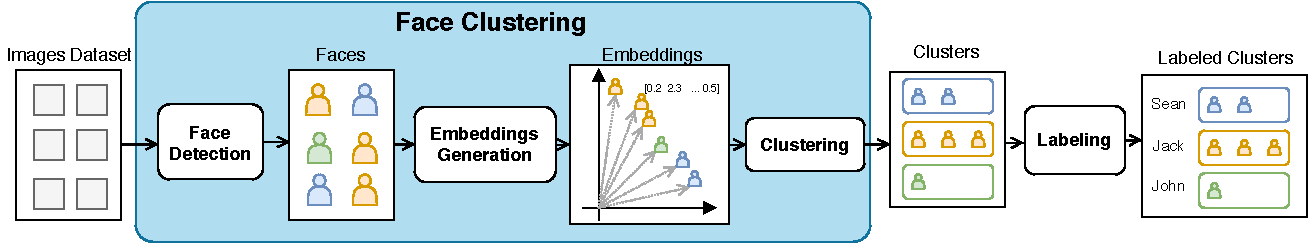
\includegraphics[width=\textwidth]{img/webmedia/labeled_clusters.pdf}
    \caption{Labeled clusters process.}
    \label{fig:labeled_clusters}
\end{figure*}

The \textit{Face Detection} step uses an object detection model for detecting faces in each of its images.
%%
This model is responsible for returning the bounding boxes of the faces present in the image, specified by the $x$ and $y$ axes coordinates of the upper-left corner and of the lower-right corner of the rectangle that establishes the visual limits that encapsulate each face. 
%%
With these bounding boxes, we can isolate and extract the bounded images, obtaining a dataset composed of images of faces only.


The objective of the \textit{Embeddings Generation} step is to represent each face image as a vector space in $\mathbb{R}^{n}$.
%%
To achieve that, it processes each of the faces generated in the previous step through a CNN, generating embeddings. 
%%
An embedding is a representation of the input in a lower dimensionality space.

In the \textit{Clustering} step, we group embeddings and, consequently, faces that are close in the embedding space using a clustering algorithm. 
%%
The clustering process should produce a partition of the dataset, i.e., each generated cluster represents a specific person, and the union of all clusters covers the whole dataset.

Finally, in the \textit{Labeling} step, we assign labels~(identities) to represent the clusters.
%%
Using this pipeline, instead of having to label every single face for constructing a labeled dataset, it is only necessary to label each generated cluster.
%%
Consequently, all the faces present in a cluster are assigned to the same label.
%%
At the end of this step, we have a dataset of labeled clusters.

\subsubsection{Cluster Matching for Video Face Recognition}
\label{subsec:cluster_match}

\begin{figure*}[!ht]
    \centering
    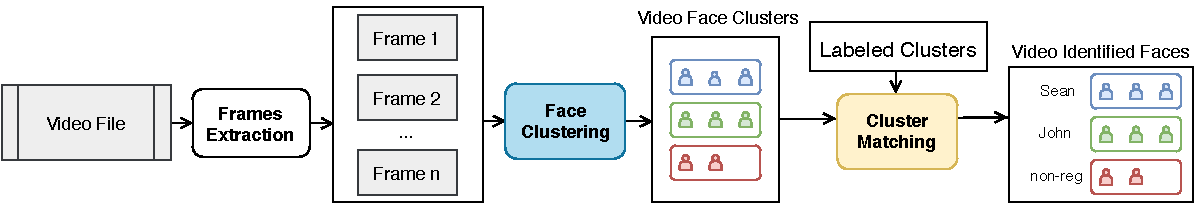
\includegraphics[width=\textwidth]{img/webmedia/video_face_recognition.pdf}
    \caption{Cluster-matching based method for automatic face recognition in video files.}
    \label{fig:cluster_matching}
\end{figure*}

This phase aims at recognizing the faces present in a video file. 
%%
It is divided in three steps: \emph{frames extraction}, \emph{face clustering} and \emph{cluster-matching}.
%%
Figure \ref{fig:cluster_matching} shows the pipeline we propose for this phase, described in the remainder of this subsection.

First, we perform \textit{Frames Extraction} by receiving a video file as input and extracting its frames according to a given frame rate. 
%%
These frames are used as a set of images for the next step.

Next, the \textit{Face Clustering} step, which is a macro-step that comprises the three first steps of the \emph{Labeled Clusters Generation} phase~(\emph{Face Detection}, \emph{Embeddings Generation}, and \emph{Clustering}), receives this set of images and returns a set of clusters of the faces present in the images received  (see Figure \ref{fig:labeled_clusters}).
%%
%In this phase, the input images are the frames of the video being processed.
%%
It is important to notice that this phase uses the same methods used for \emph{Labeled Clusters Generation}.
%%
Consequently, the embeddings of the faces from the video are part of the same embedding space as the data points (faces) in the labeled clusters.

Finally, the \textit{Cluster Matching} step receives the set of clusters from the video and the set of labeled clusters, which is used as a reference for recognizing the clusters (and consequently the faces) in the video.
%%
%%
We designed a method based on cluster distance for performing this recognition.

\subsection{Evaluation}

We have performed two experiments to evaluate our method. 
%%
The first evaluation aimed at measuring how well our approach of \emph{Face Clustering} performed using different combinations of CNNs and Clustering Algorithms. 
%%
The second evaluation aimed at measuring how well our approach performed on video. Each of these evaluations are describe in the following subsections.

\subsubsection{Faces Clustering Evaluation}
\label{faces_clustering_evaluation}
In the \emph{Face Detection} step, we use MTCNN~\cite{mtcnn} (Multitask
Cascaded Convolutional Networks) which is widely used for the face detection task.

For the \emph{Embeddings Generation} step, we have three candidate CNNs that were previously trained on the VGGFace2 dataset~\cite{cao2018vggface2}. The three candidate CNNs used are VGG-16~\cite{vgg16}, ResNet-50~\cite{resnet} and SeNet-50~\cite{senet}. 

For the \emph{Clustering} step, we selected the following clustering algorithms as candidates: k-Means~\cite{lloyd1982least}, affinity propagation~\cite{frey2007clustering}, and agglomerative clustering~\cite{ward1963hierarchical}.

We evaluate the models using the V-Measure~\cite{vmeasure}, which is an entropy-based measure that computes how successfully the criteria of homogeneity and completeness have been satisfied. This metric is extensively used for comparing clustering solutions and has been used in different domain fields such as biology~\cite{bio1}, computational linguistics~\cite{nlp1}, and document engineering~\cite{doceng}.
%%
The homogeneity score is perfect when a clustering algorithm assigns only those data points that are members of a single class to a single cluster, so that the entropy is zero in each cluster. The Completeness score is symmetrical with respect to homogeneity, and it is perfect when a clustering assigns all data points that are members of the same class to a single cluster.

Table \ref{tab:results_clustering} shows the homogeneity, completeness, and V-Measure for each combination of CNN and clustering algorithm.

\begin{table}[!ht]
\small
\centering
\caption{Results of the evaluation of the clusters created by each combination of CNN and clustering algorithms.}
\begin{tabular}{@{}ccccc@{}}
\toprule
\textbf{CNN} & \textbf{Clustering} & \textbf{$h$} & \textbf{$c$} & \textbf{$V_1$} \\ \midrule
                  & KM                  & 0.9665                     & 0.9675                      & 0.9670             \\
ResNet-50         & AP                  & 0.0000                     & 1.0000                      & 0.0000             \\
                  & AC                  & 0.9821                     & 0.9798                      & 0.9810             \\ \midrule
                  & KM                  & 0.9725                     & 0.9726                      & 0.9725             \\
SeNet-50          & AP                  & 0.9859                     & 0.9558                      & 0.9706             \\
                  & \textbf{AC}         & \textbf{0.9862}            & \textbf{0.9833}             & \textbf{0.9847}    \\ \midrule
                  & KM                  & 0.8340                     & 0.8415                      & 0.8378             \\
VGG-16            & AP                  & 0.0000                     & 1.0000                      & 0.0000             \\
                  & AC                  & 0.8899                     & 0.8929                      & 0.8914             \\
\end{tabular}
\label{tab:results_clustering}
\vspace{-1em}
\end{table}
From Table \ref{tab:results_clustering}, one can conclude that the best combination of CNN and clustering algorithm was SeNet-50 with Agglomerative Clustering.
%%
For this reason, we decided to use SeNet-50 for the \emph{Embeddings Generation} phase and the Agglomerative Clustering algorithm for the \emph{Clustering} phase.

\subsubsection{Video Face Recognition Evaluation}

To evaluate our complete pipeline, we selected videos that contain only registered people (videos \emph{a} to \emph{d}), videos with both registered and non-registered people (videos \emph{e} to \emph{i}) and videos with only non-registered people (videos \emph{j} to \emph{m}).

For performing the face identification on a video file, we first extract its frames using a frame rate of 1fps.
%%
For each of the frames, we extract the faces present on it using MTCNN~\cite{mtcnn}. 
%%
Then, for each face identified, we resize it to 224x244, extract its embedding using SeNet-50 and cluster these faces using the Agglomerative Clustering algorithm.

Next, we perform the \emph{Cluster Matching} with the labeled clusters and the video face clusters.
%%
At the end of this process, each face present on the video is labeled either with the name of a registered person or as non-registered.

%%
We evaluate our method by the Precision~(Prec), Recall (Rec), and F1-Score for the faces in the video. 
%%
As usual, the Precision is defined as the percentage of detected faces that our method correctly labels, 
%%
the Recall gives the percentage of faces that our method correctly labels among all faces in the video, and 
%%
the F1-score represents an overall performance metric based on the  harmonic mean of the precision and recall.
\begin{table}[!ht]
\centering
\small
\caption{Results using the proposed approach in videos.}
\vspace{-1em}
\label{tab:results_videos}
\begin{tabular}{@{}cccccccc@{}}
\toprule
\textbf{Video} & \textbf{\#P} & \textbf{\#R} & \textbf{\#F} & \textbf{\#EM} & \textbf{Rec.} & \textbf{Prec.} & \textbf{F1} \\ 
\multicolumn{8}{c}{\cellcolor[HTML]{C0C0C0}{\color[HTML]{000000} videos with only registered people}}\\
a%\footnote{https://youtu.be/QjTZ\_TE1U\_g} 
& 1 & 1  & 105 & 105 & 100.000\% & 100.000\% & 100.000\%  \\
b%\footnote{https://youtu.be/4D5GGR3g\_7c}
& 1 & 1  & 80  & 79  & 100.000\% & 98.765\%  & 99.379\%   \\
c%\footnote{https://youtu.be/quYNTUsOTb8}
& 1 & 1 & 60  & 59   & 100.000\% &	98.113\% & 99.048\%   \\
d%\footnote{https://youtu.be/eB6kJYaoxHc}
& 2 & 2  & 226 & 226 & 100.000\% & 100.000\% & 100.000\%  \\ 
\multicolumn{8}{c}{\cellcolor[HTML]{C0C0C0}{\color[HTML]{000000} videos with both registered and non-registered people}}\\
e%\footnote{https://youtu.be/j07yExfJ4mA}
& 2 & 1  & 101 & 99  & 100.000\% & 98.113\%  & 99.048\%   \\
f%\footnote{https://youtu.be/Db2I1uUyDlE}
& 2 & 1  & 650 & 650 & 100.000\% & 100.000\% & 100.000\%  \\
g%\footnote{https://youtu.be/sf56sWeiMyo}
& 8 & 1  & 201 & 190 & 96.471\%  & 96.850\%  & 96.660\%   \\
h%\footnote{http://youtu.be/dYAFXogdqW4}
& 4 & 1  & 231 & 215 & 98.097\%  & 98.514\%  & 98.305\%   \\
i%\footnote{http://youtu.be/NHglWWOKmc4}
& 2 & 1  & 88  & 88  & 100.000\% & 100.000\% & 100.000\%  \\ 
\multicolumn{8}{c}{\cellcolor[HTML]{C0C0C0}{\color[HTML]{000000} videos with only non-registered people}}\\
j%\footnote{https://youtu.be/UH0nTHb6OdY}
& 6 & 0  & 625 & 617 & 99.551\%  & 99.551\%  & 99.551\%   \\
k%\footnote{http://youtu.be/wHN5vYlJ-Vk}
& 2 & 0  & 231 & 228 & 100.000\% & 98.872\%  & 99.433\%   \\
l%\footnote{http://youtu.be/WwRdjf4eEgk}
& 2 & 0  & 131 & 121 & 99.482\%  & 95.522\%  & 97.462\%   \\
m%\footnote{http://youtu.be/3dIVdsiPDH8}
& 1 & 0  & 225 & 222 & 99.556\%  & 99.115\%  & 99.335\%   \\
\bottomrule
\end{tabular}
\vspace{-1em}
\end{table}
We also count the number of exact frames match (\#EM). It corresponds to the number of frames (\#F) for which our method correctly labeled all the faces that appears. 
%%
Table \ref{tab:results_videos} shows the results we obtained, the number of different people in each video~(\emph{\#P}), and the number of people who are present in the labeled clusters~(\emph{\#R}).

One can observe that our method is able to correctly classify the faces of people that are present in the labeled clusters while also being able to tell when a person is not registered in the labeled clusters.

Our method can also be used to generate metadata in video files indicating the people that appear in it.
%%
Figure \ref{fig:timeline_pol} shows the first 12 seconds of \emph{Video d}~(detailed in Table \ref{tab:results_videos}) where two identified Brazilian politicians are shown in each frame with its respective colored cluster.

\begin{figure}[!ht]
    \centering
    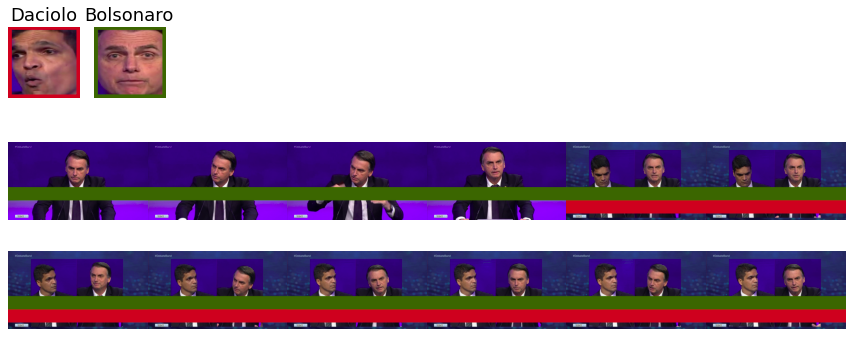
\includegraphics[width=0.6\linewidth]{img/webmedia/timeline_pol.png}
\vspace{-1em}
    \caption{Timeline with tagged frames by their clusters of registered people}
    \label{fig:timeline_pol}
\end{figure}

Besides being able to recognize people in video files, by using face embeddings and clustering, we can detect the frames where the same person appears without even knowing who the person is or if he/she is in the labeled clusters.
%%
This can be done by following the pipeline described in Figure \ref{fig:cluster_matching} up to the \emph{Face Clustering} step, obtaining the video face clusters.
%%
Figure \ref{fig:timeline} shows the first 24 seconds of \emph{Video j}~(detailed in Table \ref{tab:results_videos}) with the frames tagged with the clusters identified in each frame, where each color represents a cluster.

\begin{figure}[!ht]
    \centering
    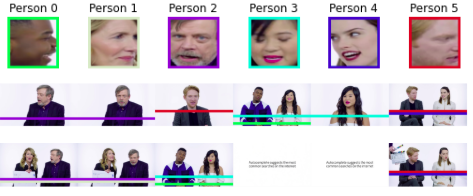
\includegraphics[width=0.6\linewidth]{img/webmedia/timeline2.png}
    \caption{Timeline with tagged frames by their clusters of non-registered people}
    \label{fig:timeline}
\end{figure}
\section{A Clustering-Based Method for Automatic Educational Video Recommendation Using Deep Face-Features of Lecturers}

Following the approach described in Section \ref{webmedia}, in \cite{mendes2020ISM}, we used actors face clustering for recommending videos that share the presence of the same actors. 
%%
This work aimed at recommending educational video content based on lecturers' presence.
To do that, we take advantage of face detection methods.
More precisely, we detect lecturers in a video taken as a reference and perform a clustering based on the face of these lecturers in different videos.
Given these clusters, we extract their \textit{centroids} (explained in Section~\ref{sec:ism_method}), and perform another clustering step for creating a relationship between videos that share the presence of the same lecturers.
Finally, we rank the recommended videos based on the amount of time the referenced lecturers were present.
A particular feature of this approach is that it can be done without supervision, allowing for new videos to be automatically analyzed.

%As we obtained the best results with the combination SeNet-50 with Agglomerative Clustering in \cite{mendes2020cluster}, we used this same combination in \cite{mendes2020ISM}. 

\begin{figure}[!ht]
    \centering
    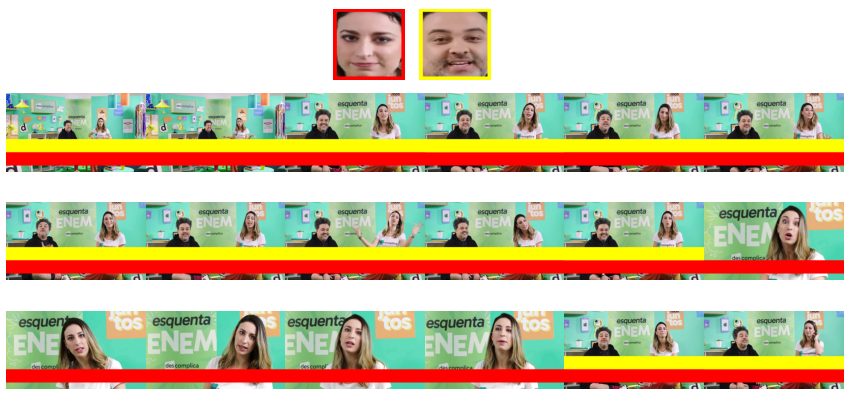
\includegraphics[width=0.75\textwidth]{img/ism/educational_timeline2.png}
    \caption{Timeline with tagged frames by their clusters~(actors) present.}
    \label{fig:timeline2}
\end{figure}



%In that work, we used actors face clustering in 98 videos and around 72\% of the faces went to the correct clusters. Figure \ref{fig:timeline2} shows part of the timeline of one of the videos tagged with colors representing the color of each actor present.


\subsection{Method}
\label{sec:ism_method}

Our method intends to recommend educational videos based on the lecturers that appear in each video, so that, when a person watches a video, other videos containing the same lecturers are recommended.
For didactic purposes we decided to divide our exposition in two phases: (i)~\emph{video representation} and (ii)~\emph{video recommendation}, which are described in Sections~\ref{subsec:video_representation} and \ref{subsec:video_recommendation} respectively.

\subsubsection{Video Representation}
\label{subsec:video_representation}

\begin{figure*}[!ht]
  \centering
  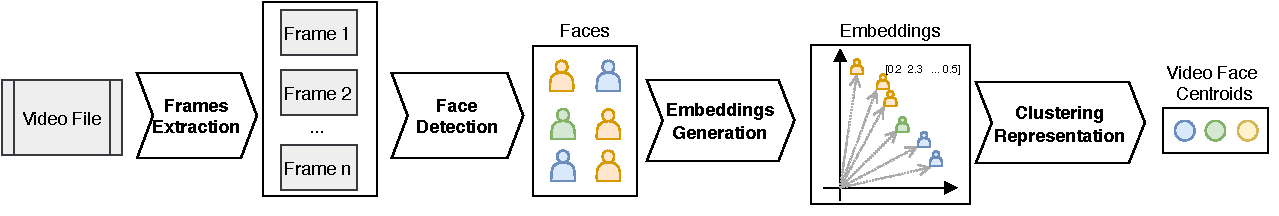
\includegraphics[width=\linewidth]{img/ism/video_clustering_line.pdf}
  \caption{Video representation process with lecturers face centroids. }
  \label{fig:video_clustering}
\end{figure*}

The objective of this phase is to represent each video with vectors~(centroids) of the lecturers that appear on it. 
Fig. \ref{fig:video_clustering} shows the pipeline we propose for this phase, described in the remainder of this subsection.
It is divided into four steps: \emph{Frames Extraction}, \emph{Face Detection}, \emph{Embeddings Generation} and \emph{Clustering Representation}.

The steps of this process are the same used in Figure \ref{fig:cluster_matching} up to the \emph{Face Clustering} step, obtaining the video face clusters.
%%
The difference here is that the \emph{Clustering Representation} returns the centroids of the clusters found.
%%
By the end of this phase, we have each video in the dataset represented by its centroids where, ideally, each centroid represents a lecturer present in the video.


\subsubsection{Video Recommendation}
\label{subsec:video_recommendation}

This phase aims at recommending videos by the lecturers present in it and in the other videos.
It is divided in two steps: \emph{Centroids Clustering} and \emph{Ranking}, as depicted in Fig. \ref{fig:video_recommendation}.

\begin{figure*}[!ht]
  \centering
  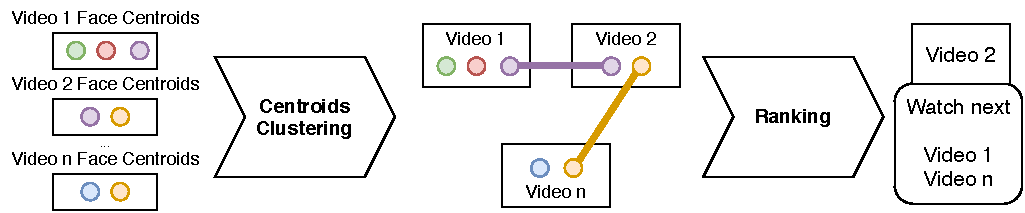
\includegraphics[width=0.8\linewidth]{img/ism/video_recommendation.pdf}
  \caption{Video Recommendation process.}
  \label{fig:video_recommendation}
\end{figure*}

First, we gather the centroids from the videos of the dataset as one single set and perform the \textit{Centroids Clustering}.
%%
By doing that, we group centroids from the same lecturer that are in different videos. For instance, in Fig. \ref{fig:video_recommendation}, one can see that the \emph{purple lecturer} is present in both Videos 1 and 2, while the \emph{orange lecturer} is present in both Videos 2 and n. By the end of this step, we have the group $L$ of lecturers present in the dataset of videos $V$, and we can also denote $L_v$ as the group of lecturers present in video $v$.

Next, based on these relationships among different videos, we perform \textit{Ranking}, by recommending videos in which lecturers of the current video are present. 
%%
For doing that, we compute a similarity score using the presence of the lecturers in the current video and the presence of these same lecturers in the other video.
%%
Let $p_{l,v}$ denote the percentage of frames in which the lecturer $l \in L_v$ is present in video $v \in V$. For each video $v \in V$ and $u \in V-v$ we compute a score of similarity $S_{v,u}$.

\vspace{-1em}
\begin{equation}
  S_{v,u} = \sum_{l~\in~L_v}{p_{l,v}\cdot{p_{l,u}}}
\end{equation}

Finally, using this score, for each video $v$ we compute a ranking $R_{v}$ where $R_{v,i}$ denotes the \emph{i-greatest} $S_v$ and $R_{v,i}\ge~R_{v,i+1}$ for all $i~\in~1...n_v$, where $n_v$ is the number of videos $u$ in which $S_{v,u}>~0$. 
%%
In this way, the more lecturers a video have in common with the reference video, and the more time these lecturers are present in both videos, the higher the video is positioned in the ranking of the reference video.  

By the end of this phase, we have a ranking of recommended videos for each video in the dataset.
%%
It is important to notice that our method is unsupervised and does not require the information of the lecturers in advance.
%%
Consequently, we do not store any information regarding the identity of the lecturers, respecting their privacy.

\subsection{Evaluation}

For representing the video files in the dataset, we start by performing \emph{Frames Extraction} for each video file using a frame rate of 1 frame per second~(fps). 
%%
Next, in the \emph{Face Detection} step, we use MTCNN \cite{mtcnn} (Multitask
Cascaded Convolutional Networks). 
%%
Once we have detected the faces of lecturers in the video frames, we perform \emph{Embeddings Generation} using SeNet-50 \cite{senet}.
%%
Finally, in the \emph{Clustering Representation} step, we used the Ward Agglomerative Clustering~\cite{ward1963hierarchical}.
%%
The choice for the combination SeNet-50 with the Agglomerative Clustering algorithm comes from the fact that this combination returned the best results in the evaluation described in Section \ref{faces_clustering_evaluation}.

For performing the video recommendation task, we gather the centroids~(that represent each lecturer in the video) from all videos in the dataset. Next, we perform the process described in Section \ref{subsec:video_recommendation}.

We evaluate our approach based on the relevance of the videos recommended. A video is considered relevant to another if they have at least one lecturer in common.
%%
To verify that, we use the information of the lecturers' presence available on our dataset.
%%
%%
To evaluate our ranking, for each video we compute the Average Precision~(AP), that evaluates how well a ranking of recommendations is based on each element's relevancy. 
%%
This metric penalizes more a ranking if a non-relevant element is recommended in the first positions than if it was in the last ones.

In order to prevent outliers from having much influence in the recommendation (e.g. a person that is not a lecturer -- and not relevant to the video -- and appears for a short amount of time), we evaluated different thresholds of presence intervals in a video for a person to be considered as ``present'' when computing the score for the ranking. 
%%
In this way, a $p_{l,v}$ lesser than the threshold is considered as $0$.
%%
Besides the Average Precision, we also compute the mean value of the recall~(MeanR), precision~(MeanP), and F1-Score~(MeanF1) for the recommendation generated for each of the videos, without considering the positioning of these videos in the rankings.

One can observe from Table \ref{tab:results} that the precision clearly increased with the use of the threshold.
%%
Different from the precision, the recall decreased with the increase of the threshold. It means that with a greater threshold more videos that should be recommended were not chosen by our method.
%%
It is important to notice that these two metrics~(precision and recall) do not consider the ordering of the recommendations.
%%
Different from them, the Mean Average Precision~(mAP) has high values for all thresholds, especially because the score for computing the ranking takes into consideration the percentage of time that a person appears in the reference and recommended videos.
%%
Then, we can conclude that our proposed approach for ordering the recommended videos tends to recommend more suitable videos first with a high mAP$\approx0.99$.

\begin{table}[!ht]
\small
\centering
\caption{Results with different thresholds of presence.}
\label{tab:results}
\begin{tabular}{ccccccccc}
\hline
\textbf{Thershold} & \textbf{MeanR} & \textbf{MeanP} & \textbf{MeanF1}  & \textbf{mAP} \\ \hline
0\%                & 0,88851        & 0,64681        & 0,70971          & 0,98641      \\
5\%                & 0,88851        & 0,69923        & 0,74930          & 0,98642      \\
10\%               & 0,88742        & 0,83165        & 0,84306          & 0,98643      \\
15\%               & 0,88289        & 0,90265        & 0,88450          & 0,98884      \\
20\%               & 0,86130        & 0,93645        & 0,89218          & 0,99000      \\
25\%               & 0,85805        & 0,95718        & 0,90046          & 0,99165     
\end{tabular}
\end{table}

\section{Automatic Subtitles Positioning in 360-Video}

The recent popularization of omnidirectional cameras and Head-Mounted-Displays (HMDs) has increased the amount of 360-video content available \cite{mendes2020authoring}. These videos are spherical visual signals that allow the viewer to look around a full 360-degree view of a scene from a specific point. When using HMDs, at each instant in time, the viewer is presented with a viewport that is updated as the viewer moves their head. This type of content, especially when consumed through Virtual Reality~(VR) devices (HMDs included), can provide immersive experiences in which the user has a strong feeling of presence when compared with the use of traditional media \cite{montagud_culture_2020}. Due to this increasing popularity, we decided to investigate the usage of spatiotemporal localization of actors in 360-video.

Nowadays, the most common way for representing and transmitting 360-video is using an equirectangular projection~\cite{yang2018object}. With the equirectangular projection, each sphere point is defined by two angles~\cite{snyder1987map}: \emph{latitude}~$\theta \in [-90^{\circ}, +90^{\circ}]$ and \emph{longitude}~$\phi \in [-180^{\circ}, +180^{\circ}]$. This kind of projection creates challenges for image processing and computer vision algorithms, especially to the convolution-based ones because of the severe distortions in areas vertically distant from the center of the image~(see Figure \ref{fig:equirectangular_proj}).

\begin{figure}[!ht]
\centering
    \begin{subfigure}{0.47\linewidth}
        \centering
        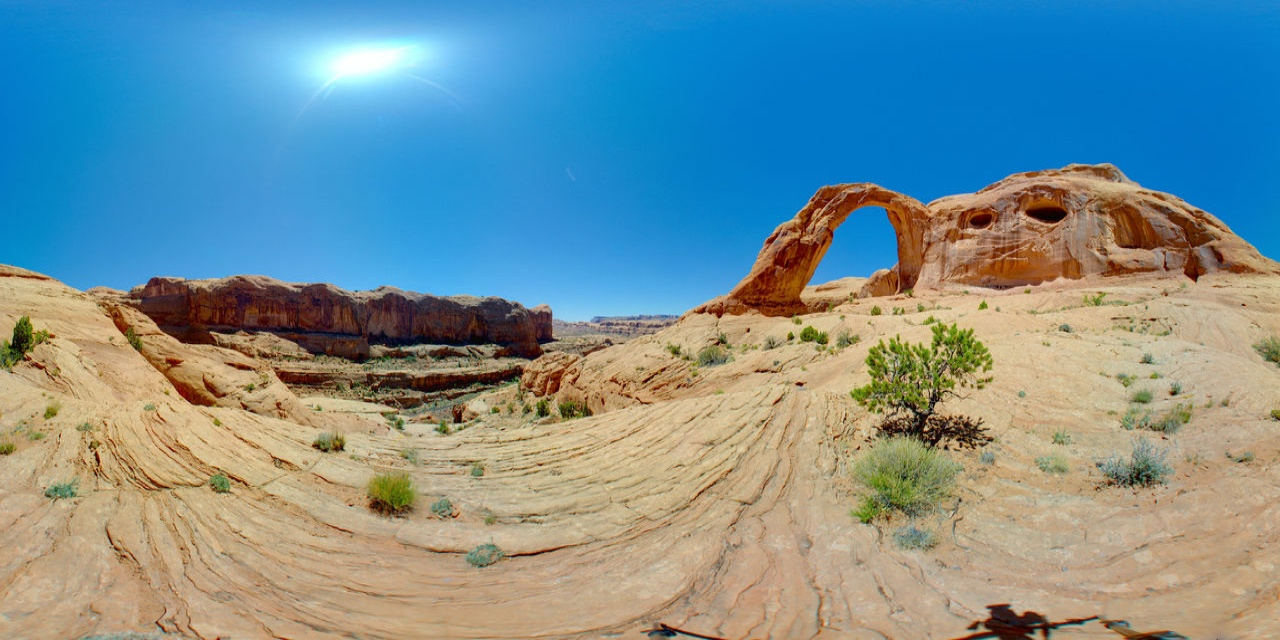
\includegraphics[width=1\textwidth]{img/image (9).jpg}
        \caption{Outdoor equirectangular image.}
        \label{subfig:out_equi}
    \end{subfigure}\hfill
    \begin{subfigure}{0.47\linewidth}
        \centering
        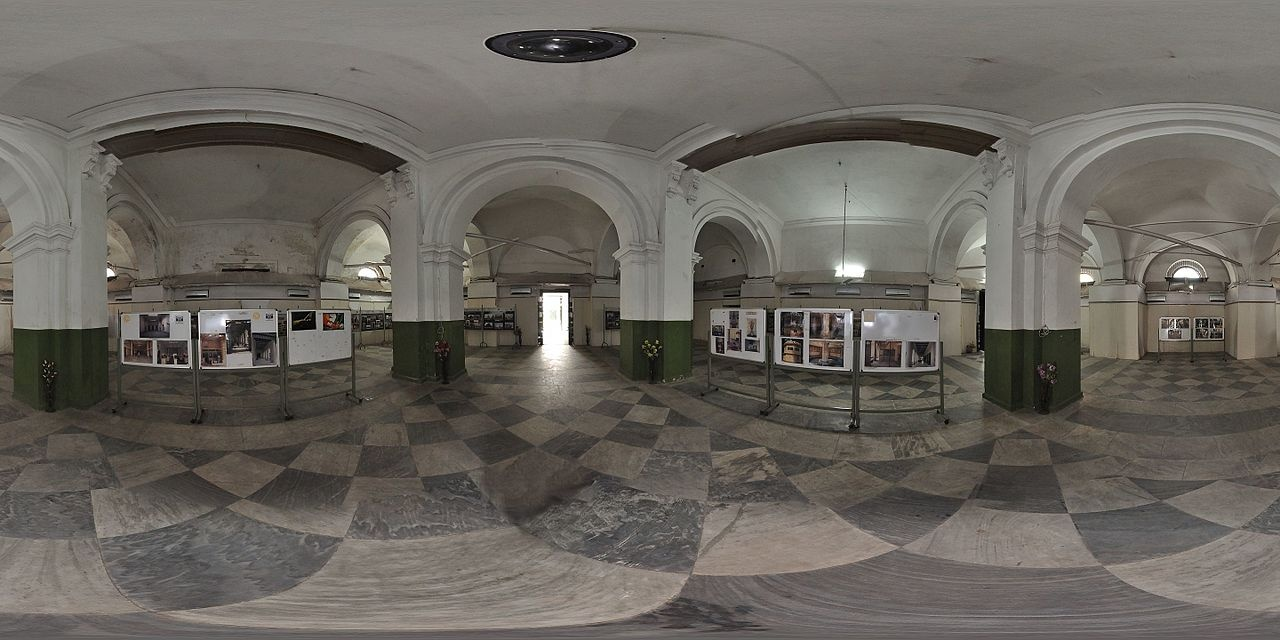
\includegraphics[width=1\textwidth]{img/image (10).JPG}
        \caption{Indoor equirectangular image.}
        \label{subfig:in_equi}
    \end{subfigure}

\caption{Examples of 360-images represented through equirectangular projection.}
\label{fig:equirectangular_proj}
\end{figure}

Due to these distortions, we adapted the steps of our methods that use traditional CNNs: \emph{Face Detection} and \emph{Embeddings Generation}. These adaptations are described in Sections \ref{subsec:360_adaptations}. In Section \ref{subsec:dynamic_subtitles}, we describe how these adaptations can be used for subtitles positioning in 360-videos.

\subsection{Face Detection and Embeddings Generation in 360-Videos}
\label{subsec:360_adaptations}

Because of the distortions present on the equirectangular projection, we opted for elaborating a solution based on viewports extraction. A viewport is defined by its center, in polar coordinates~(lat, long), and its field of view~(FoV). Figure \ref{fig:viewports} shows viewports extracted at different polar coordinates from Figure \ref{subfig:out_equi}.

\begin{figure}[!ht]
    \centering
    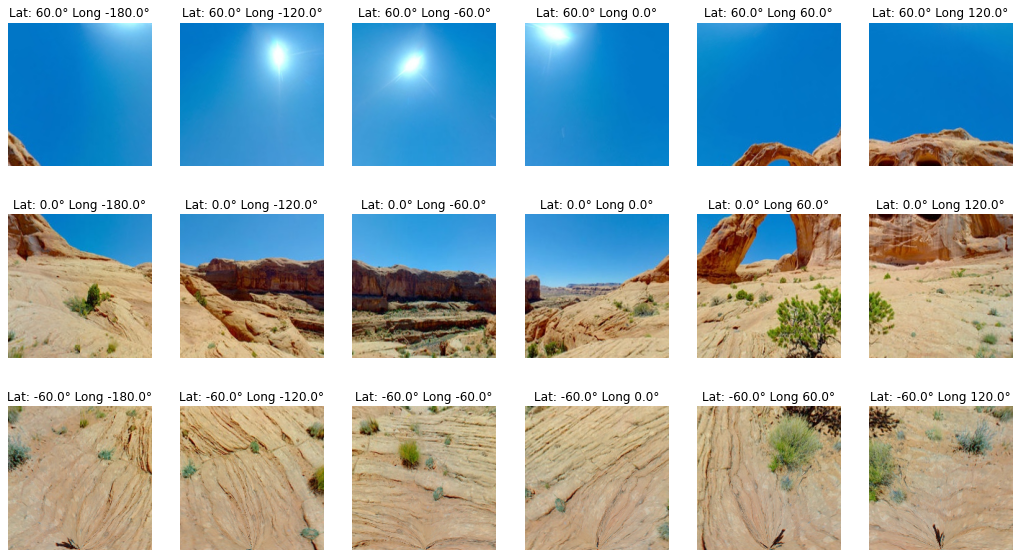
\includegraphics[width=1\textwidth]{img/viewports.png}
    \caption{Viewports extracted at different polar coordinates with $FoV = 60^{\circ}$}
    \label{fig:viewports}
\end{figure}

For each viewport, we apply a face detection model. 
Then, we project the faces detected bounding boxes back to the equirectangular image. For doing that for a given bounding box, we project the four corners and the mean point of each edge~(8 points in total). Therefore, in the equirectangular image, we deal with polygons instead of bounding boxes, due to the distortions introduced. As different viewports may intersect and cover part of the same region in an image, we apply Non-maximum Supression~(NMS), eliminating intersected detections within a given threshold. One of the main advantages of this approach is that we can use face detection models trained in regular images, since distortions are reduced with the use of viewports. In order to test this approach, we have created a synthetic dataset.

Due to the lack of datasets for face detection in equirectangular images, we created a synthetic dataset based on the FDDB dataset~\cite{fddbTech}, a popular benchmark for face detection evaluation containing 2845 images and 5171 faces. We collected 19 indoor and outdoor equirectangular images, from Google Images,\footnote{https://www.google.com/imghp} ESO,\footnote{https://www.eso.org/public} and PxHere.\footnote{https://pxhere.com}
For each image in the FDDB dataset, we randomly chose a latitude, longitude and equirectangular image to project it. For each face present on that image, we projected the bounding box to a polygon exactly as mentioned in the viewport process. Figure \ref{fig:fddb_proj} shows an example of an image from FDDB projected in the polar coordinates \emph{lat} $ = -60^{\circ}$ \emph{long} $= 0^{\circ}$ to an equirectangular image.

\begin{figure}[!ht]
\centering
    \begin{subfigure}{0.4\linewidth}
        \centering
        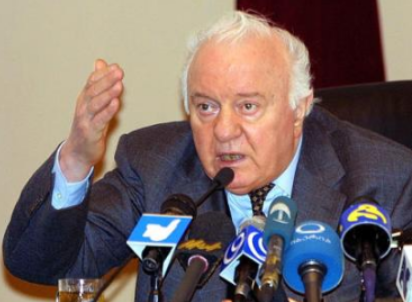
\includegraphics[height=10em]{img/face_pre.png}
        \caption{FDDB image example.}
        \label{subfig:face_pre}
    \end{subfigure}\hfill
    \begin{subfigure}{0.55\linewidth}
        \centering
        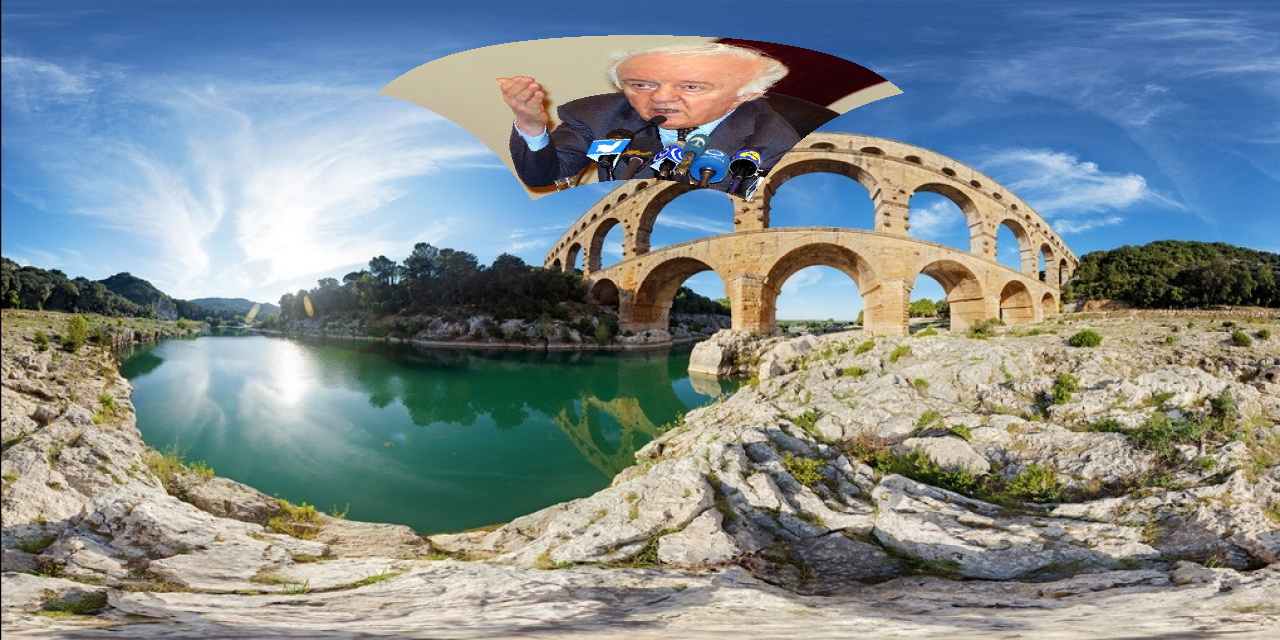
\includegraphics[height=10em]{img/face_pos.png}
        \caption{Projection example of FDDB image.}
        \label{subfig:face_pos}
    \end{subfigure}

\caption{FDDB image projection to Equirectangular image.}
\label{fig:fddb_proj}
\end{figure}

After eliminating repeated detections with NMS, we perform \emph{Embeddings Generation} using the faces detected in the viewports~(with reduced distortions) instead of using its equivalent in the original equirectangular video frame.

For this part of our work, we have defined the following remaining task.

\begin{itemize}
    \item \textbf{T 1}: Model test using MTCNN and MTCNN with viewports~(80\% complete).
\end{itemize}

\subsection{Authoring Model for Interactive 360-Videos}
\label{subsec:dynamic_subtitles}

In \cite{mendes2020authoring}, we proposed a model for authoring interactive 360° video. In such a model, we can define interactive 360° video that are presented together with additional information attached to it, such as image, text and spatial audio. The positioning of such additional information is defined by their polar coordinates, start time and duration. Moreover, we can also configure behaviours depending on where the user is looking. For instance, we can define that a text moves with the user's head motion and is always visible or that such text is placed at fixed position if it is in the field of view of the user. Besides the design of such a model, we developed a player that follows the definitions of our model and is able to play interactive 360° video defined by it. Then, we can use the results obtained from the previous phase to define the positioning of subtitles according to the actors positioning using our player.
\section{Contributions}
\label{sec_contritutions}
 As collateral contributions of this research, three papers have been published in relevant multimedia conferences \cite{mendes2020cluster, mendes2020authoring, mendes2020ISM}. In \cite{mendes2020authoring}, we have developed an authoring model and a player for interactive 360º video, enabling subtitles positioning. In \cite{mendes2020cluster}, we have evaluated video face clustering together with a cluster-matching method for video face recognition. In \cite{mendes2020ISM}, we have used video face clustering and the presence of actors in different video as a mean for recommending educational videos.
 
\section{Expected Contributions}
\label{sec_expected}
In our dissertation, we aim at exploring the usage of spatiotemporal localization of actors and its applications in video. We intend to investigate its usage in the tasks of video face recognition and recommendation. Moreover, we will examine the applicability of this method in the authoring process of interactive 360-video with dynamic subtitles based on actors localization.


\section{Schedule}
\label{sec_schedule}
Table \ref{tab:schedule} presents the schedule we propose for completing the remainder tasks of this research.

\definecolor{darkgray}{RGB}{180,180,180}
\definecolor{gray}{RGB}{205,205,205}
\definecolor{lightgray}{RGB}{218,218,218}
\definecolor{lightlightgray}{RGB}{238,238,238}

\definecolor{darkred}{RGB}{204,0,0}
\definecolor{red}{RGB}{224,102,102}
\definecolor{lightred}{RGB}{244,199,195}

\definecolor{darkmagenta}{RGB}{61,133,198}
\definecolor{magenta}{RGB}{111,168,220}
\definecolor{lightmagenta}{RGB}{166,206,242}

% \definecolor{mark}{RGB}{224,102,102} %red
\definecolor{mark}{RGB}{111,168,220} %magenta

\definecolor{white}{RGB}{255,255,255}

\arrayrulecolor{white}
% \arrayrulecolor{darkgray}
\setlength\tabcolsep{3.0pt} % space between the text and the left/right border. Default Value = 6.0pt

\begin{table} [!ht]
  \centering
  \caption{Schedule of this dissertation proposal.}
  \label{tab:schedule}

  \begin{tabularx}{21em}{|p{6em}|p{5em}|p{5em}|p{5em}}
 
  \rowcolor{darkgray} & 
  \multicolumn{3}{|c|}{\textbf{2021}}\\ 
  
  \rowcolor{gray}
  \multicolumn{1}{|c|}{\multirow{-2}{*}{\cellcolor{darkgray}\textbf{Tasks}}} & 
  \multicolumn{1}{|c|}{\textbf{May}} & 
  \multicolumn{1}{|c|}{\textbf{Jun}} & 
  \multicolumn{1}{|c|}{\textbf{Jul}}\\
%   \hline
%%%%%%%%%%%%%%%%%%%%%%%%%%%%%%%%%%%%%%%%%%%%%%%%%%%%%%%%%%%%%%%%%%%%%%%%%%%%%%%%%%%%%%%%%%%%%%%%%%%%%%%%%%%%%%%%%%%%%%%%%%%%%%%%%%%%%%
  \rowcolor{lightgray}
       & \cellcolor{mark} &  &\\
  \rowcolor{lightgray}
    \multicolumn{1}{|c|}{\multirow{-1}{*}{T1}}
       & \cellcolor{mark} & &\\
  \rowcolor{lightgray}  
   & \cellcolor{mark} & & \\
%   \hline
%%%%%%%%%%%%%%%%%%%%%%%%%%%%%%%%%%%%%%%%%%%%%%%%%%%%%%%%%%%%%%%%%%%%%%%%%%%%%%%%%%%%%%%%%%%%%%%%%%%%%%%%%%%%%%%%%%%%%%%%%%%%%%%%%%%%%%
  \rowcolor{lightlightgray}
  &  & \cellcolor{mark}  & \cellcolor{mark}\\
  \rowcolor{lightlightgray}
    \multirow{-2}{*}{Dissertation} 
    &  & \cellcolor{mark}  & \cellcolor{mark}\\
  \rowcolor{lightlightgray}
    \multirow{-2}{*}{Writing} 
    &  & \cellcolor{mark}  & \cellcolor{mark}\\
%   \hline
%%%%%%%%%%%%%%%%%%%%%%%%%%%%%%%%%%%%%%%%%%%%%%%%%%%%%%%%%%%%%%%%%%%%%%%%%%%%%%%%%%%%%%%%%%%%%%%%%%%%%%%%%%%%%%%%%%%%%%%%%%%%%%%%%%%%%%
  \rowcolor{lightgray}
  &  &  & \cellcolor{mark}\\
  \rowcolor{lightgray}
    \multirow{-2}{*}{Dissertation} 
  &  &  & \cellcolor{mark}\\
  \rowcolor{lightgray}
  \multirow{-2}{*}{Presentation}
  &  &  & \cellcolor{mark}\\
\arrayrulecolor{darkgray}    

%   \end{tabular}
  \end{tabularx}
\end{table}

% Development of model instantiation
% Preliminary evaluation 
% Evaluation 
% Evaluation data analysis
% Thesis writing
% Thesis defense

\newpage
% \addcontentsline{toc}{section}{Referências}
\addcontentsline{toc}{section}{References}

\bibliographystyle{sbc}
% \bibliographystyle{plainnat}
\bibliography{sbc-template}

\end{document}
